\begin{frame}
  \frametitle{Visualisierung}
  \Wider{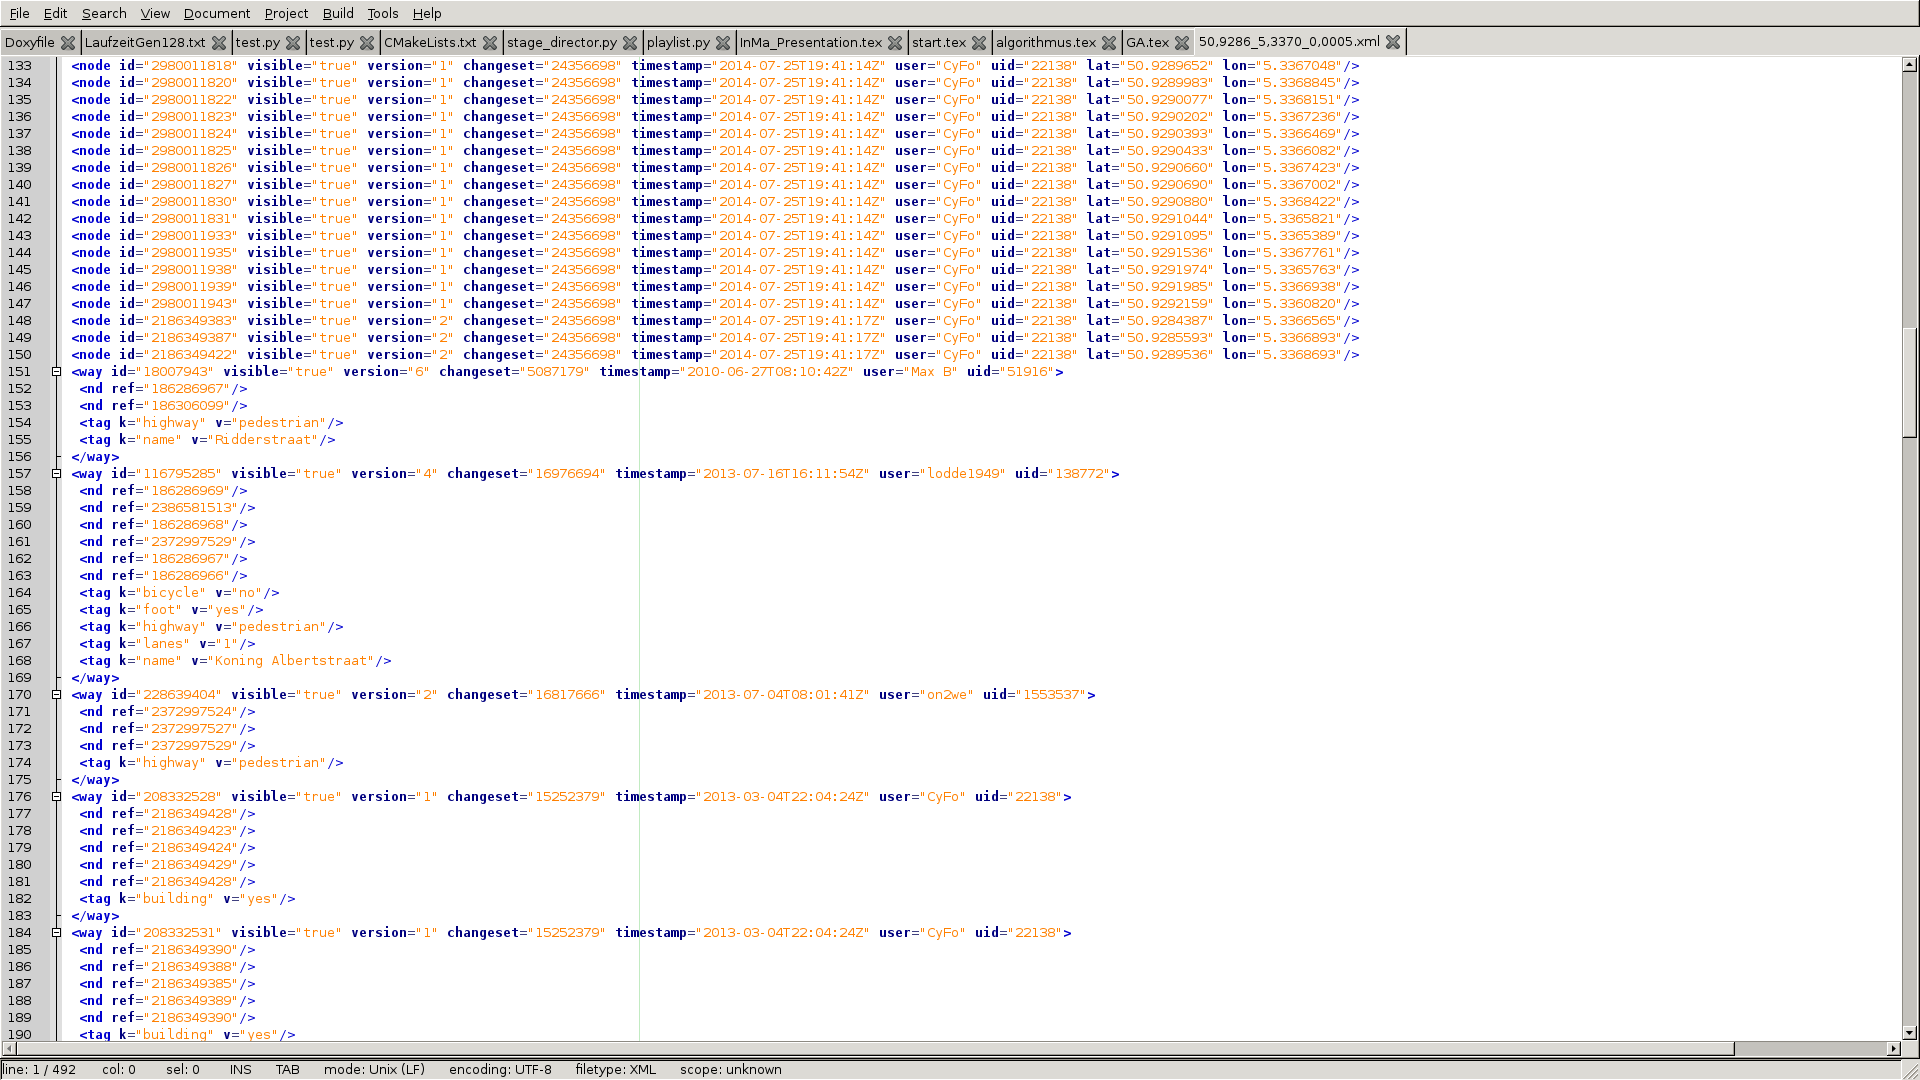
\includegraphics[width=\textwidth]{XML}}
\end{frame}

\begin{frame}
  \frametitle{Visualisierung}
%%%%%%%%%%%%%%%%%%%%%%%%%%%%%%%%%%%%%%%%%%%%%%%%%%%%%%%%%%%%%%%%%%%%%%%%%%%%%%%%
  % Hier ein Bild von unserer Visualisierungsklasse
  % danach ein Frame mit Bild, bei dem die Tags von einem Teil vergrößert sind (Picture in Picture)
  % danach ein Frame mit Bild, bei dem zusätzlich noch die richtige Lösung und unser Tipp farbig eingezeichnet sind
  % vielleicht hier dann erst mal unsere Idee darstellen.
  % danach ein Frame mit Bild, bei dem gezeigt wird, dass die Tags jetzt noch zusätlich "entfernung" und "gewichtete Entfernung"
%%%%%%%%%%%%%%%%%%%%%%%%%%%%%%%%%%%%%%%%%%%%%%%%%%%%%%%%%%%%%%%%%%%%%%%%%%%%%%%%
\end{frame}

\begin{frame}
  \frametitle{Coverage}
  \begin{equation*}
    Coverage = \frac{Area_{intersection}}{max(Area_{guesspolygon},Area_{loesungspolygon})}
  \end{equation*}
\\
  \begin{equation*}
    Coverage \in {0..1}
  \end{equation*}
%%%%%%%%%%%%%%%%%%%%%%%%%%%%%%%%%%%%%%%%%%%%%%%%%%%%%%%%%%%%%%%%%%%%%%%%%%%%%%%%
% Vielleicht hier 3 kleine Beispiele für Coverage.
% 0: intersection = null
% 1: intersection = lösung  % oder beliebige andere
% 0.1: Lösung ist 1/10 von guess groß und liegt in ihr drinne
%%%%%%%%%%%%%%%%%%%%%%%%%%%%%%%%%%%%%%%%%%%%%%%%%%%%%%%%%%%%%%%%%%%%%%%%%%%%%%%%
\end{frame}

\begin{frame}
  \frametitle{Naiver Ansatz}
%%%%%%%%%%%%%%%%%%%%%%%%%%%%%%%%%%%%%%%%%%%%%%%%%%%%%%%%%%%%%%%%%%%%%%%%%%%%%%%%
% Coverage Wert für den Naiven Ansatz Einfügen
%%%%%%%%%%%%%%%%%%%%%%%%%%%%%%%%%%%%%%%%%%%%%%%%%%%%%%%%%%%%%%%%%%%%%%%%%%%%%%%%
  \begin{center}
  \huge{Coverage = ...}
  \end{center}
\end{frame}

\begin{frame}
  \frametitle{Gewichteter Ansatz}
%%%%%%%%%%%%%%%%%%%%%%%%%%%%%%%%%%%%%%%%%%%%%%%%%%%%%%%%%%%%%%%%%%%%%%%%%%%%%%%%
% Coverage Wert für den Naiven und ersten Ansatz Einfügen
%%%%%%%%%%%%%%%%%%%%%%%%%%%%%%%%%%%%%%%%%%%%%%%%%%%%%%%%%%%%%%%%%%%%%%%%%%%%%%%%
  \begin{center}
  \huge{Coverage = ...}
  \end{center}
  \begin{center}
  Naive Coverage = ...
  \end{center}
\end{frame}

\begin{frame}
  \frametitle{Unvollständige Daten}
%%%%%%%%%%%%%%%%%%%%%%%%%%%%%%%%%%%%%%%%%%%%%%%%%%%%%%%%%%%%%%%%%%%%%%%%%%%%%%%%
% Bild von unserer Image-Klasse mit einem unvollständigen Datensatz (am besten wieder 38)
%%%%%%%%%%%%%%%%%%%%%%%%%%%%%%%%%%%%%%%%%%%%%%%%%%%%%%%%%%%%%%%%%%%%%%%%%%%%%%%%
\end{frame}

\begin{frame}
  \frametitle{Umgebungspolygon}
%%%%%%%%%%%%%%%%%%%%%%%%%%%%%%%%%%%%%%%%%%%%%%%%%%%%%%%%%%%%%%%%%%%%%%%%%%%%%%%%
% Erklärung zu dem Umkreispolygon und dem anschließenden schneiden.
%%%%%%%%%%%%%%%%%%%%%%%%%%%%%%%%%%%%%%%%%%%%%%%%%%%%%%%%%%%%%%%%%%%%%%%%%%%%%%%%
\end{frame}

\begin{frame}
  \frametitle{Umgebungspolygon}
%%%%%%%%%%%%%%%%%%%%%%%%%%%%%%%%%%%%%%%%%%%%%%%%%%%%%%%%%%%%%%%%%%%%%%%%%%%%%%%%
% Bild von unserer Image-Klasse mit einem unvollständigen Datensatz und dem geschnittenen Ansatz (am besten wieder 38)
%%%%%%%%%%%%%%%%%%%%%%%%%%%%%%%%%%%%%%%%%%%%%%%%%%%%%%%%%%%%%%%%%%%%%%%%%%%%%%%%
\end{frame}

\begin{frame}
  \frametitle{Vollständiger Ansatz}
%%%%%%%%%%%%%%%%%%%%%%%%%%%%%%%%%%%%%%%%%%%%%%%%%%%%%%%%%%%%%%%%%%%%%%%%%%%%%%%%
% Coverage Wert für den vollständigen und ersten Ansatz Einfügen
%%%%%%%%%%%%%%%%%%%%%%%%%%%%%%%%%%%%%%%%%%%%%%%%%%%%%%%%%%%%%%%%%%%%%%%%%%%%%%%%
  \begin{center}
  \huge{Coverage = ...}
  \end{center}
  \begin{center}
  Vorheriger Coverage = ...
  \end{center}
\end{frame}

\begin{frame}
  \frametitle{Sonstige Verbesserungen}
  \begin{itemize}
    \item Partielle Gebäude zu einem zusammen gefügt
    \item OSM-Daten zwischengespeichert
    \item GPS-Daten aus Bildern auslesen.
%%%%%%%%%%%%%%%%%%%%%%%%%%%%%%%%%%%%%%%%%%%%%%%%%%%%%%%%%%%%%%%%%%%%%%%%%%%%%%%%
% Weitere Verbesserungen die wir gemacht haben, aber nicht groß erklären wollen.
%%%%%%%%%%%%%%%%%%%%%%%%%%%%%%%%%%%%%%%%%%%%%%%%%%%%%%%%%%%%%%%%%%%%%%%%%%%%%%%%
    \item ...
  \end{itemize}
\end{frame}

\begin{frame}
    \frametitle{rules.xml Format}
    %Content goes here
\end{frame}
